\documentclass[a4paper,10pt]{article}

%Packages
\usepackage{txfonts}
\usepackage{titlesec}
\usepackage[utf8]{inputenc}
\usepackage[T1]{fontenc}
\usepackage{geometry}
\usepackage{graphicx}
\usepackage{lipsum}
\usepackage{multicol}
\usepackage{fancyhdr}
\usepackage{hyperref}
\usepackage{float}
\usepackage{setspace}
\usepackage{caption}
\usepackage{booktabs}

% PAGE LAYOUT
\geometry{a4paper, top=18mm, bottom=18mm, textwidth=185mm}
\setlength{\columnsep}{6mm}
\setlength{\parindent}{0pt}

\titleformat{\section}
{\normalfont\bfseries}
	{\thesection.}{0.5em}{}
\titleformat{\subsection}
	{\normalfont\itshape}
	{\thesubsection.}{0.5em}{}

\pagestyle{fancy}
\renewcommand{\footrulewidth}{0pt}
\fancyhf{}
\rhead{
\includegraphics[scale=0.4]{Images/hepia_simple.png}}
\rfoot{\textit{\today}}
\cfoot{\thepage}

\captionsetup{
  font=footnotesize,
  labelsep=colon
}

\begin{document}

\begin{multicols*}{2}
[
\begin{center}
\vspace*{0mm}
{\large
AI in Healthcare data -- Module 1\\
\vspace{3mm}
Data Preparation, Summarization, Visualization, Reduction and \\
Diagnostic Performance Analysis of a Prostate Cancer Cohort
}\\
\vspace{8mm}
Guilhem Rozier Vilardell\footnote{\textit{\href{mailto:guroz26@student.sdu.dk}{guroz26@student.sdu.dk}}}
\\
\vspace{3mm}
\footnotesize{
\textit{AI in Healthcare Summer Camp -- Data Preparation, Summarization, Visualization and Reduction}
}\\
\vspace{9mm}
\end{center}
\rule{\linewidth}{0.4pt}
\onehalfspacing
\textbf{Abstract}\\
Three raw datasets describing a prostate cancer (PC) cohort -- demographic/clinical records, biochemical laboratory values, and coded comorbidity diagnoses -- were cleaned, type-corrected, and merged into a single analysis-ready dataset (1{,}159 patients, 25 variables). Missing biochemical values were imputed and the resulting panel was summarized descriptively and by correlation structure. Prostate-specific antigen (PSA) was then evaluated as a diagnostic marker of metastasis at two fixed cutoffs and across its full range via ROC analysis (AUC = 0.670), and the ten biochemical markers were reduced to three principal components (PC1--PC3, 69.3\% cumulative variance) using PCA. A multivariable logistic regression model was then built on the full merged dataset, refined by backward elimination (21 candidate predictors reduced to 13), and validated with 10-fold stratified cross-validation, reaching a mean AUC of 0.855 (accuracy 0.783) -- a substantial improvement over PSA alone. Alternative classifiers (SVM, random forest, regularized logistic regression) performed within 1--2 points of the final logistic model, and a single-patient explanation was produced with LIME. Results show PSA has moderate, cutoff-dependent discriminative power; that the biomarker panel is compressible with limited information loss; and that combining biomarkers, comorbidities and demographics substantially improves discrimination over PSA alone, at the cost of added complexity and reduced interpretability.\\
\noindent\textit{Keywords:} prostate cancer, PSA, missing data, ROC curve, PCA, biomarker panel, logistic regression, cross-validation, LIME\\
\rule{\linewidth}{0.4pt}
]
\singlespacing

\tableofcontents

\setlength{\parskip}{1pt}
\columnbreak
% INTRODUCTION
\section{Introduction}
Prostate cancer (PC) is a disease that happens to a large proportion of the population. The goal of this research is to explore the use of AI to help in the diagnosis of prostate cancer.\\
Until now, diagnosis and follow-up rely on heterogeneous data: clinical records, laboratory records, and medical history. The first step in any data analysis is to prepare the data for modeling.\\
Before any of this data can support diagnostic or prognostic modelling, it must be inspected and understood. To help us we will manipulate the data by type-corrected, checked for missingness, merged into a coherent structure, and -- where the number of correlated biomarkers is large -- reduced to a smaller, more tractable set of components.\\
This report covers this data cleaning phase, feature selection and classification. Data preparation, summarization, visualization and diagnostic performance and data reduction of the AI in Healthcare summer camp.\\
The two questions that interest us are: (i) how should missing and heterogeneous data from three separate sources be prepared into a single reliable cohort table, and (ii) how well does prostate-specific antigen (PSA), alone, discriminate patients who go on to develop metastasis, and can the wider biomarker panel be compressed without losing much information.

% DATA
\section{Data}

Three source files, identified by patient \texttt{ID}, were provided.

\textbf{DATASET1 -- clinical data}: civil status, family history of cancer, metastasis status (outcome), and three date fields (first PC diagnosis, metastasis diagnosis, birth date).

\textbf{DATASET2 -- laboratory data}: ten numeric laboratory markers (monocyte, urea, lymphocyte, thrombocyte, erythrocyte, albumin, creatinine, globulin, PSA, coagulation factor).

\textbf{DATASET3 -- medical history}: one row per diagnosed condition per patient, using condition codes (diabetes, hearing loss, hypercholesterolaemia, hypertension, osteoporosis, urinary retention).

% DATA PREPARATION AND RESULTS
\section{Data Preparation and Results}

The first step is to understand what does this data represent? do the values make sense? are there any missing values? are the data types correct?\\
The second step is to prepare the data for analysis.

\subsection{Type correction}
\textbf{Method:} In DATASET1, civil status, cancerfamily and metastasis were re-typed from integer to categorical, and the three date columns were parsed as datetimes. DATASET2's dtypes were already appropriate and left unchanged. DATASET3 was transformed from code-based entries to binary columns.

\textbf{Result:} The type correction ensured that categorical variables were properly encoded for analysis, date fields were in a usable datetime format, and the medical history was converted to a binary indicator format suitable for regression.

\subsection{Missing data handling and imputation}
\textbf{Method:} DATASET1's only missingness was in the metastasis-diagnosis date (738/1{,}159 = 63.7\% missing). It's expected since patients without metastasis have no such date. A filtered check confirmed zero patients with \texttt{metastasis=1} and a missing date, i.e. no unexplained missingness. DATASET2 showed scattered missingness across biochemical markers (0.3--14.1\% per column, worst in lymphocyte), visualized with a missingness bar chart and matrix (Fig.~\ref{fig:missbar} and \ref{fig:missmat}). Most of the histograms (Fig.~\ref{fig:hist}) appear skewed and present outliers, with the exceptions being monocyte (top left corner), thrombocyte (top right corner) and erythrocyte (first column, second row), whose distributions appear quite balanced and symmetrical. Therefore, median imputation was chosen as most suitable for the majority of the biochemical markers.

\begin{figure}[H]
\centering
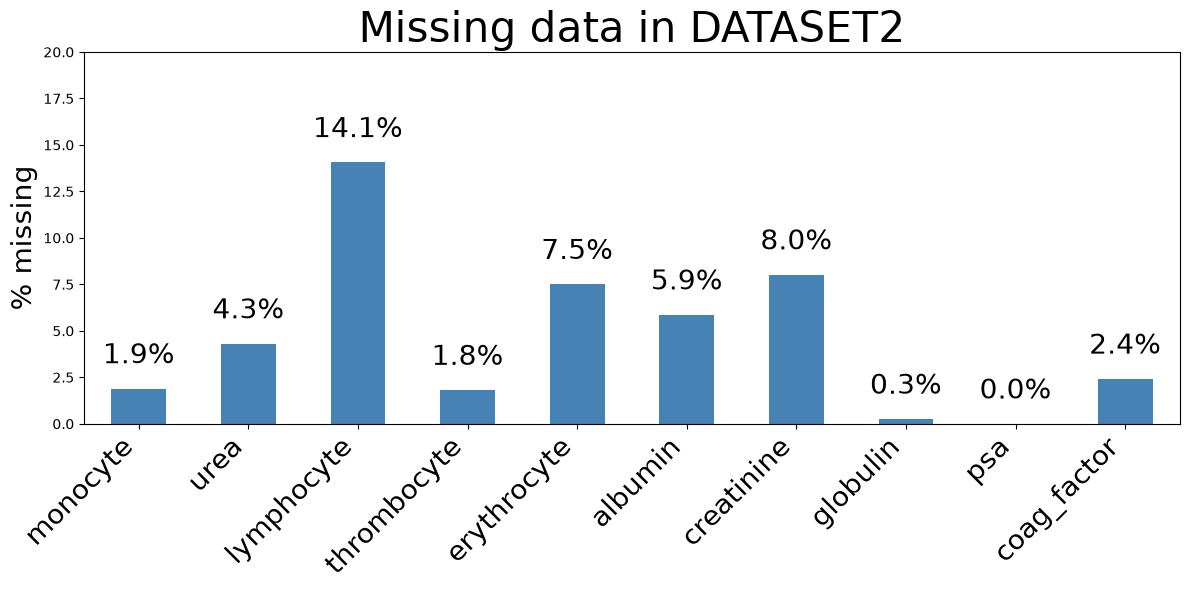
\includegraphics[width=\linewidth]{Images/missing_bar.png}
\caption{Missing-value percentage per biochemical variable, DATASET2.}
\label{fig:missbar}
\end{figure}

\begin{figure}[H]
\centering
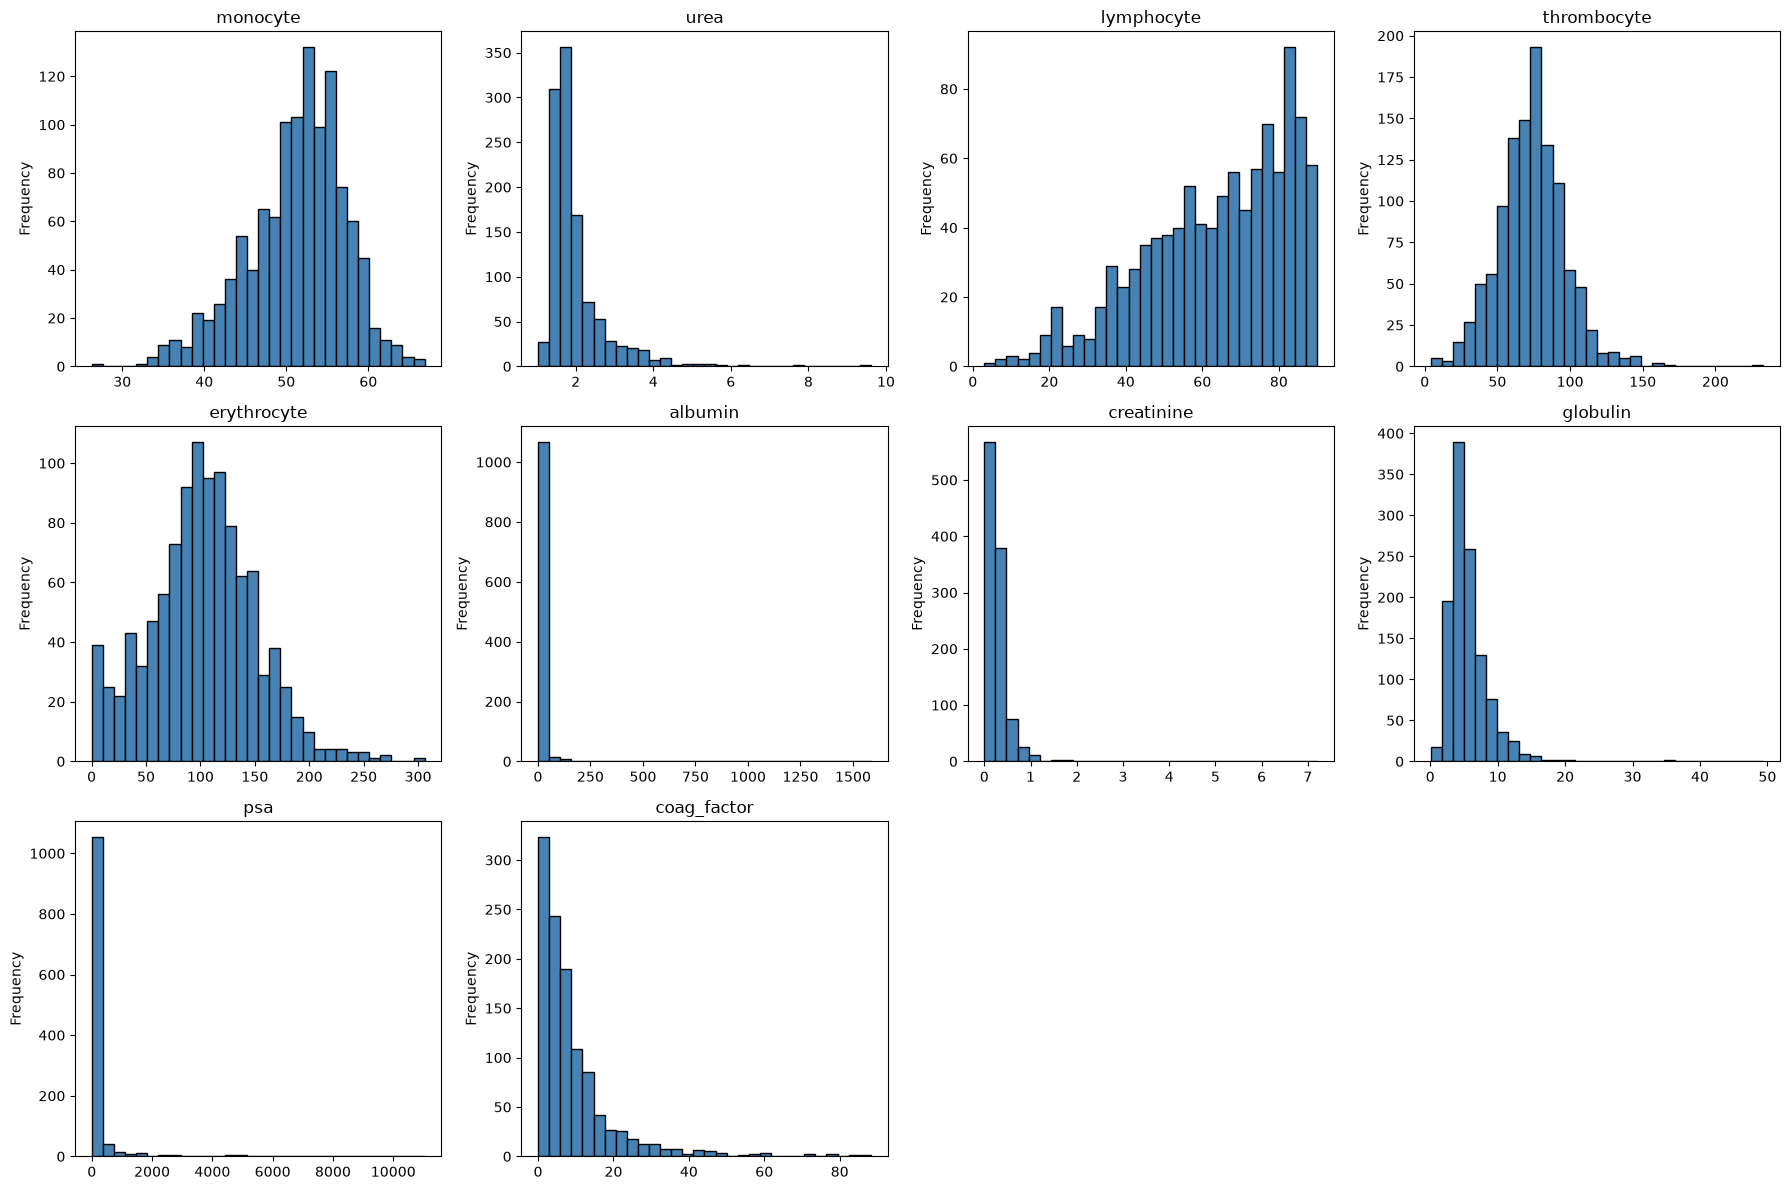
\includegraphics[width=\linewidth]{Images/biomarker_hist.png}
\caption{Distribution of the ten biochemical markers (DATASET2), used to select an imputation method.}
\label{fig:hist}
\end{figure}

\textbf{Result:} Missingness in DATASET2 is modest overall (0.3--14.1\%) and, per Fig.~\ref{fig:missmat}, scattered rather than block-patterned -- supporting the use of simple imputation over multiple imputation or case deletion.

\subsection{Recoding, reshaping, and merging}
\textbf{Method:} DATASET3's six codes were mapped to disease labels and pivoted from long format (one row per diagnosis) to wide format, one row per patient, one binary column per disease. DATASET1, DATASET2, and the wide disease table were left-joined on \texttt{ID} (base = DATASET1). Post-merge, disease columns with \texttt{NaN} (patient absent from DATASET3, i.e. no diagnosis on record) were set to 0.

\textbf{Result:} \texttt{DATASET123} (1{,}159 $\times$ 25) combines clinical, laboratory and medical history information per patient. The left-join on the DATASET1 base guarantees no patient is lost even when a source table lacks an entry for them; filling missing disease flags with 0 encodes "no diagnosis on record" rather than "unknown," which is the appropriate default for a comorbidity registry built from positive diagnostic codes only.

\subsection{Patient characteristics}
Table~\ref{tab:characteristics} summarizes the cohort derived from DATASET1.

\begin{table}[H]
\centering
\caption{Patient characteristics (N = 1{,}159).}
\label{tab:characteristics}
\begin{tabular}{lr}
\toprule
Variable & Value \\
\midrule
Age at PC diagnosis (yr) & 74.3 $\pm$ 8.7 \\
Age at metastasis (yr)$^{*}$ & 78.9 $\pm$ 8.5 \\
Metastasis: yes & 421 (36.3\%) \\
Metastasis: no & 738 (63.7\%) \\
Family history of cancer: yes & 623 (53.8\%) \\
Family history of cancer: no & 536 (46.2\%) \\
Civil status: married/cohabiting & 808 (69.7\%) \\
Civil status: single/divorced/widowed & 351 (30.3\%) \\
\bottomrule
\end{tabular}\\
\footnotesize{$^{*}$computed on the 421 patients with metastasis.}
\end{table}

Roughly one in three patients in the cohort developed metastasis. The age at metastasis diagnosis is on average $\sim$4.6 years older than age at initial PC diagnosis, consistent with metastasis typically occurring after initial diagnosis rather than at presentation.

\subsection{Correlation structure}
\textbf{Method:} Pairwise Pearson correlations between the ten biomarkers were computed and visualized as a heatmap (Fig.~\ref{fig:corr}) to check for redundancy before PCA.

\begin{figure}[H]
\centering
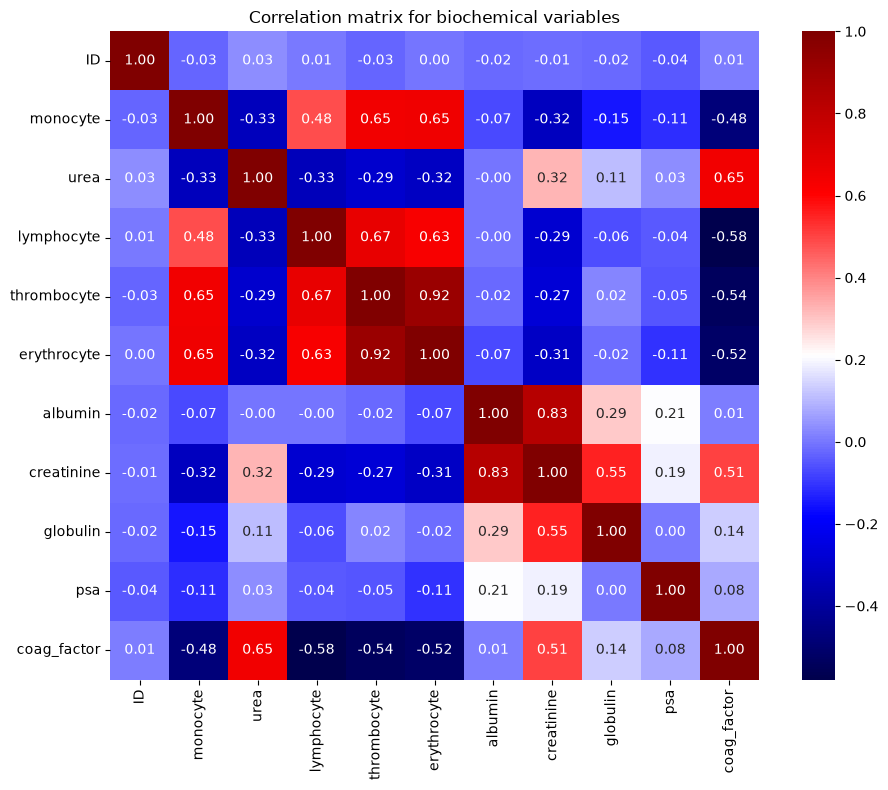
\includegraphics[width=\linewidth]{Images/corr_heatmap.png}
\caption{Correlation matrix of the ten biochemical markers.}
\label{fig:corr}
\end{figure}

\textbf{Result:} The correlation heatmap (Fig.~\ref{fig:corr}) shows mostly weak pairwise correlations, with only a few moderate associations plausibly linked to shared hematologic/renal physiology; no pair approaches $|r|\approx1$, so variable dependencies is not a major concern for downstream modelling.

\subsection{PSA diagnostic performance}
\textbf{Method:} Metastasis was used as the ground-truth label. Two fixed PSA cutoffs (20 and 100~ng/mL) were tested by building binary test-result columns and computing sensitivity, specificity and accuracy against the confusion matrix. A full receiver operating characteristic (ROC) analysis was then run using PSA as a continuous score, and the optimal cutoff was located two ways: (i) the Youden index, and (ii) class-size-weighted maximum accuracy.

\textbf{Result:} Table~\ref{tab:psa} reports performance at the two pre-specified PSA thresholds.

\begin{table}[H]
\centering
\caption{PSA diagnostic performance at two fixed cutoffs.}
\label{tab:psa}
\begin{tabular}{lcc}
\toprule
 & PSA $>$20 ng/mL & PSA $>$100 ng/mL \\
\midrule
Sensitivity & 0.596 & 0.323 \\
Specificity & 0.672 & 0.867 \\
Accuracy & 0.645 & 0.670 \\
\bottomrule
\end{tabular}
\end{table}

The low cutoff maximizes sensitivity (catches more true metastatic cases, more false alarms); the high cutoff maximizes specificity (few false alarms, misses roughly two-thirds of metastatic cases). Accuracy is similar for both ($\sim$0.65--0.67) because it is pulled toward the majority (non-metastatic) class, illustrating why accuracy alone is a poor criterion for choosing a cutoff in an imbalanced cohort.

\subsection{ROC analysis and optimal cutoff}
\begin{figure}[H]
\centering
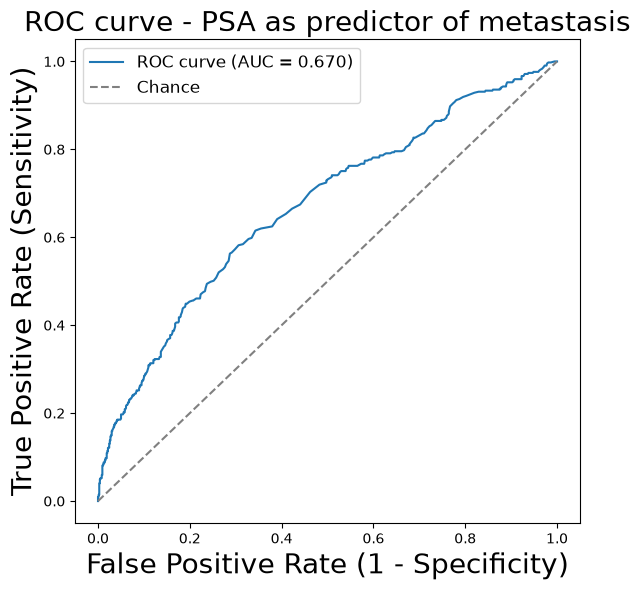
\includegraphics[width=\linewidth]{Images/roc_curve.png}
\caption{ROC curve for PSA as a continuous predictor of metastasis. AUC = 0.670.}
\label{fig:roc}
\end{figure}

AUC = 0.670 indicates moderate discrimination -- better than chance (0.5) but well below what is expected of a strong single-marker test ($\gtrsim$0.9). The two cutoff-selection criteria disagree substantially: the Youden index selects 23~ng/mL (sensitivity 0.582, specificity 0.694), close to the pre-specified 20~ng/mL cutoff, while maximum accuracy selects 134~ng/mL (accuracy 0.679), close to the pre-specified 100~ng/mL cutoff. This mirrors the fixed-cutoff result: Youden weighs sensitivity and specificity equally, while class-weighted accuracy favours the majority (non-metastatic) class and therefore specificity.

\subsection{Principal Component Analysis}
\textbf{Method:} The ten biomarkers were standardized (zero mean, unit variance, since PCA is scale-sensitive) and decomposed with PCA. Components were retained using the eigenvalue$>1$ (Kaiser) criterion.

\textbf{Result:} By the eigenvalue$>1$ criterion, 3 components were retained (eigenvalues 3.90, 1.95, 1.10; the 4th drops to 0.93), jointly explaining 69.3\% of total variance in the ten-marker panel (Fig.~\ref{fig:scree}).

\begin{figure}[H]
\centering
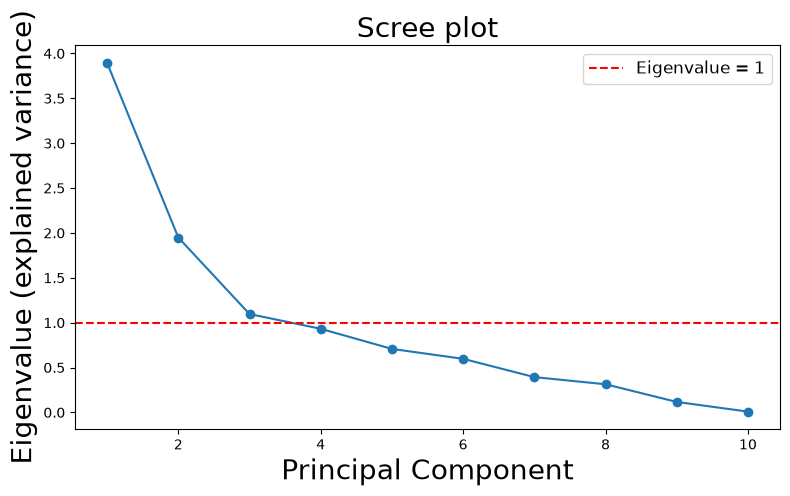
\includegraphics[width=\linewidth]{Images/scree_plot.png}
\caption{Scree plot of PCA eigenvalues, with the eigenvalue = 1 (Kaiser) cutoff.}
\label{fig:scree}
\end{figure}

Table~\ref{tab:loadings} gives the component loadings. PC1 loads positively on monocyte, lymphocyte, thrombocyte and erythrocyte and negatively on urea and coagulation factor. PC2 loads most strongly and positively on albumin and creatinine. PC3 loads most strongly and positively on PSA and negatively on urea -- a PSA-dominated axis distinct from the other two.

\begin{table}[H]
\centering
\caption{PCA component loadings (top-magnitude markers per PC).}
\label{tab:loadings}
\begin{tabular}{lrrr}
\toprule
Marker & PC1 & PC2 & PC3 \\
\midrule
monocyte     & 0.381  & 0.112  & $-$0.137 \\
urea         & $-$0.290 & $-$0.041 & $-$0.479 \\
lymphocyte   & 0.348  & 0.167  & 0.051 \\
thrombocyte  & 0.412  & 0.245  & $-$0.225 \\
erythrocyte  & 0.412  & 0.199  & $-$0.260 \\
albumin      & $-$0.132 & 0.593  & 0.248 \\
creatinine   & $-$0.323 & 0.532  & $-$0.047 \\
globulin     & $-$0.128 & 0.436  & $-$0.345 \\
psa          & $-$0.085 & 0.173  & 0.600 \\
coag\_factor  & $-$0.405 & $-$0.063 & $-$0.296 \\
\bottomrule
\end{tabular}
\end{table}

Keeping 3 of 10 markers as components (a $70\%$ dimensionality reduction) retains roughly two-thirds of the panel's variance, which is a reasonable trade-off for use as predictors in a downstream model, at the cost of losing direct clinical interpretability of any single original marker.

\subsection{Univariate logistic regression}
\textbf{Method:} Before building a multivariable model, urinary retention was tested alone as a predictor of metastasis, a hypothesis suggested by clinicians. A univariate logistic regression (\texttt{metastasis} $\sim$ \texttt{urinary\_retention}) was fitted and its coefficient converted to an odds ratio.

\textbf{Result:} Urinary retention alone was a significant predictor of metastasis (coefficient $=0.911$, $p<0.001$; odds ratio $=2.49$): a patient with urinary retention has roughly 2.5 times the odds of metastasis of one without, with no adjustment for other variables. Predicted probability of metastasis was 0.526 for patients with retention versus 0.308 for those without. $R^2$ was only 0.029, confirming retention alone explains little of the outcome's variance -- expected for a single-predictor model, and the motivation for next task. At the default 0.50 probability cutoff, this univariate model reached 65\% accuracy but only 37\% recall on the metastasis class (precision 53\%), since almost no patient's predicted probability clears 0.50 on retention status alone.

\subsection{Multiple logistic regression and collinearity}
\textbf{Method:} A multivariable model was fitted using every remaining variable in \texttt{DATASET123}, excluding \texttt{ID}, the two date columns, \texttt{birthdate}, and \texttt{age\_at\_metastasis} (defined only when \texttt{metastasis=1}). The three PCA components were also excluded from this first pass, so that a raw-biomarker model could be directly compared, via variance inflation factor (VIF), against a version using PC1--PC3 in place of the ten raw biomarkers.

\textbf{Result:} The full model (21 predictors) reached pseudo $R^2=0.320$, a large improvement over the univariate model. However, the VIF check (Table~\ref{tab:vif}) showed the raw-biomarker model does not satisfy the independence-of-predictors assumption: creatinine, albumin and coagulation factor all exceeded the VIF$=10$ problematic threshold, with globulin and thrombocyte in the 5--10 caution range. Replacing the ten raw biomarkers with PC1--PC3 dropped every VIF to $\approx$1--2, confirming that the PCA components fully resolve the collinearity, at the cost of losing direct clinical interpretability of the affected coefficients.

\begin{table}[H]
\centering
\caption{Variance inflation factor, raw-biomarker model (variables with VIF~$\geq$~5 shown).}
\label{tab:vif}
\begin{tabular}{lr}
\toprule
Variable & VIF \\
\midrule
Creatinine & 63.4 \\
Albumin & 35.4 \\
Coagulation factor & 14.7 \\
Globulin & 6.6 \\
Thrombocyte & 5.3 \\
\bottomrule
\end{tabular}
\end{table}

\subsection{Feature selection via backward elimination}
\textbf{Method:} Starting from the full raw-biomarker model of multiple logistic regression, predictors were removed one at a time -- the least significant (highest $p$-value) first -- until every remaining predictor was significant at $\alpha=0.05$.

\textbf{Result:} Backward elimination removed 8 of the 21 candidate predictors (in order: civil status, coagulation factor, hypercholesterolaemia, hearing loss, thrombocyte, globulin, the PSA$>$100 flag, creatinine), leaving 13 variables. Model fit improved slightly despite fewer parameters (AIC $\approx 1068$ vs. $\approx 1077$; pseudo $R^2$ 0.315 vs. 0.320), indicating the dropped variables contributed noise rather than signal. Notably, creatinine and coagulation factor (both flagged for high VIF) were among the first variables dropped, consistent with the collinearity finding above. At the default 0.50 cutoff, the final model's in-sample performance improved substantially over the univariate model: 79\% accuracy, 68\% recall and 72\% precision on the metastasis class (Table~\ref{tab:final_perf}).

\begin{table}[H]
\centering
\caption{Final model in-sample classification performance (0.50 cutoff).}
\label{tab:final_perf}
\begin{tabular}{lccc}
\toprule
Class & Precision & Recall & F1 \\
\midrule
No metastasis & 0.82 & 0.85 & 0.84 \\
Metastasis & 0.72 & 0.68 & 0.70 \\
\midrule
Accuracy & \multicolumn{3}{c}{0.79} \\
\bottomrule
\end{tabular}
\end{table}

\subsection{Cross-validated performance}
\textbf{Method:} The backward-elimination model was re-fit as a scikit-learn pipeline (standardization + logistic regression) and evaluated with 10-fold stratified cross-validation, so that class balance is preserved in every fold. Accuracy, sensitivity, specificity, precision, F1-score and AUC were computed per fold and averaged.

\textbf{Result:} In-sample performance is optimistic, since the model is evaluated on the same data it was fit on. Under 10-fold stratified cross-validation, mean performance was: accuracy 0.783 (SD 0.028), sensitivity 0.675 (SD 0.058), specificity 0.846 (SD 0.044), precision 0.718 (SD 0.055), F1 0.693 (SD 0.038), AUC 0.855 (SD 0.023). The low fold-to-fold standard deviation on every metric indicates the result is stable rather than an artifact of one particular train/test split. Compared to PSA alone (AUC 0.670, Section~4.5), the cross-validated multivariable model represents a substantial improvement ($+0.185$ AUC), confirming that combining biomarkers, comorbidities and demographics captures information a single continuous PSA score cannot.

\subsection{Model comparison}
\textbf{Method:} The same cross-validation scheme was used to compare four classifiers on the final variable set: logistic regression, support vector machine (SVM), random forest, and L1-regularized (LASSO) logistic regression.

\textbf{Result:} Table~\ref{tab:modelcomp} compares four classifiers on the same 13 variables under identical 10-fold cross-validation. All four land within a narrow band (accuracy 0.783--0.786, AUC 0.841--0.855); no model dominates. SVM has the highest sensitivity/F1, random forest the highest precision, and logistic regression (plain or L1-regularized) the highest AUC. Given the near-tie in performance, logistic regression's directly interpretable coefficients (odds ratios) make it the more defensible choice for a clinical decision-support context over the less transparent SVM and random forest.

\begin{table}[H]
\centering
\caption{10-fold cross-validated performance by model type.}
\label{tab:modelcomp}
\begin{tabular}{lccccc}
\toprule
Model & Acc. & Sens. & Prec. & F1 & AUC \\
\midrule
Logistic Reg. & 0.783 & 0.675 & 0.718 & 0.693 & 0.855 \\
SVM & 0.786 & 0.713 & 0.705 & 0.707 & 0.841 \\
Random Forest & 0.785 & 0.682 & 0.716 & 0.696 & 0.843 \\
Reg.\ LR (L1) & 0.783 & 0.677 & 0.717 & 0.694 & 0.855 \\
\bottomrule
\end{tabular}
\end{table}

\subsection{Model explainability with LIME}
\textbf{Method:} For a single randomly selected patient, LIME (Local Interpretable Model-agnostic Explanations) was used to identify which of that patient's variable values contributed most to their predicted probability of metastasis, and in which direction.

\textbf{Result:} For one randomly selected patient, LIME identified the family history of cancer, albumin, diabetes status, age at diagnosis and lymphocyte count as the five locally most influential variables on that patient's predicted probability, with the absence of family history and a low lymphocyte count pulling the prediction toward "no metastasis," and elevated albumin, absence of diabetes, and older age at diagnosis pulling it toward "metastasis." Whether this specific combination is clinically plausible for that patient would need to be checked against their full record; LIME explains one prediction at a time and does not generalize the pattern to other patients.

% CONCLUSION
\section{Conclusion}

\textbf{Interpretation.} A single, merged, imputed cohort table was produced from three heterogeneous sources without patient loss. PSA alone is a moderate (AUC = 0.670), not strong, discriminator of metastasis; no single cutoff is simultaneously sensitive and specific, and the "right" cutoff depends on the clinical use case (screening favours the low, high-sensitivity cutoff; confirmation favours the high, high-specificity cutoff). The ten-marker biochemical panel compresses to three interpretable components (cellular/hematologic, renal/nutritional, PSA-dominated) retaining 69.3\% of variance. Combining the raw biomarkers with demographic and comorbidity variables in a multivariable logistic regression model, refined by backward elimination and validated with 10-fold cross-validation, raises discrimination from AUC 0.670 (PSA alone) to AUC 0.855 -- a substantial gain -- while remaining fully interpretable via odds ratios, and performing on par with less transparent alternatives (SVM, random forest).

\textbf{Impact.} These outputs directly enable clinical decision support: the final logistic regression model and its odds ratios could inform a risk-stratification tool that goes well beyond a single PSA cutoff, while remaining interpretable enough for clinician review (unlike the SVM/random forest alternatives, which matched but did not exceed its performance). The ROC/Youden analysis additionally gives a defensible, data-driven single-marker cutoff for settings where only PSA is available.

\textbf{Limitations and future steps.} The mean-vs-median imputation discrepancy identified in Section~3.2 should be corrected (re-run with true median imputation and confirm downstream results are stable to the choice). The predictor set included \texttt{test\_result20} (the PSA$>$20 flag) alongside continuous PSA itself; this variable survived backward elimination and is a partial duplicate of information already in \texttt{psa} -- worth re-running without it to confirm the final model's performance does not depend on this redundancy. The diabetes coefficient in the final model was negative (protective direction), which is not obviously consistent with clinical expectations and should be treated as a hypothesis for domain-expert review rather than an established finding, since it may reflect a confound specific to this cohort rather than a real physiological effect. More broadly, this analysis is retrospective and cross-sectional: biomarkers and outcome were measured close together in time, which limits causal interpretation (e.g. whether urinary retention precedes metastasis or co-occurs with it). A prospective design -- enrolling patients at initial diagnosis before metastatic status is known, and following them longitudinally with scheduled imaging to record time-to-metastasis -- would support survival analysis (e.g. Cox proportional hazards) instead of a binary logistic outcome, better using censored data from patients who have not yet metastasized at study end, and would let the model be tested on its ability to predict future metastasis rather than correlate with already-diagnosed metastasis.

\end{multicols*}
\section{Annexe}
\begin{figure}[H]
\centering
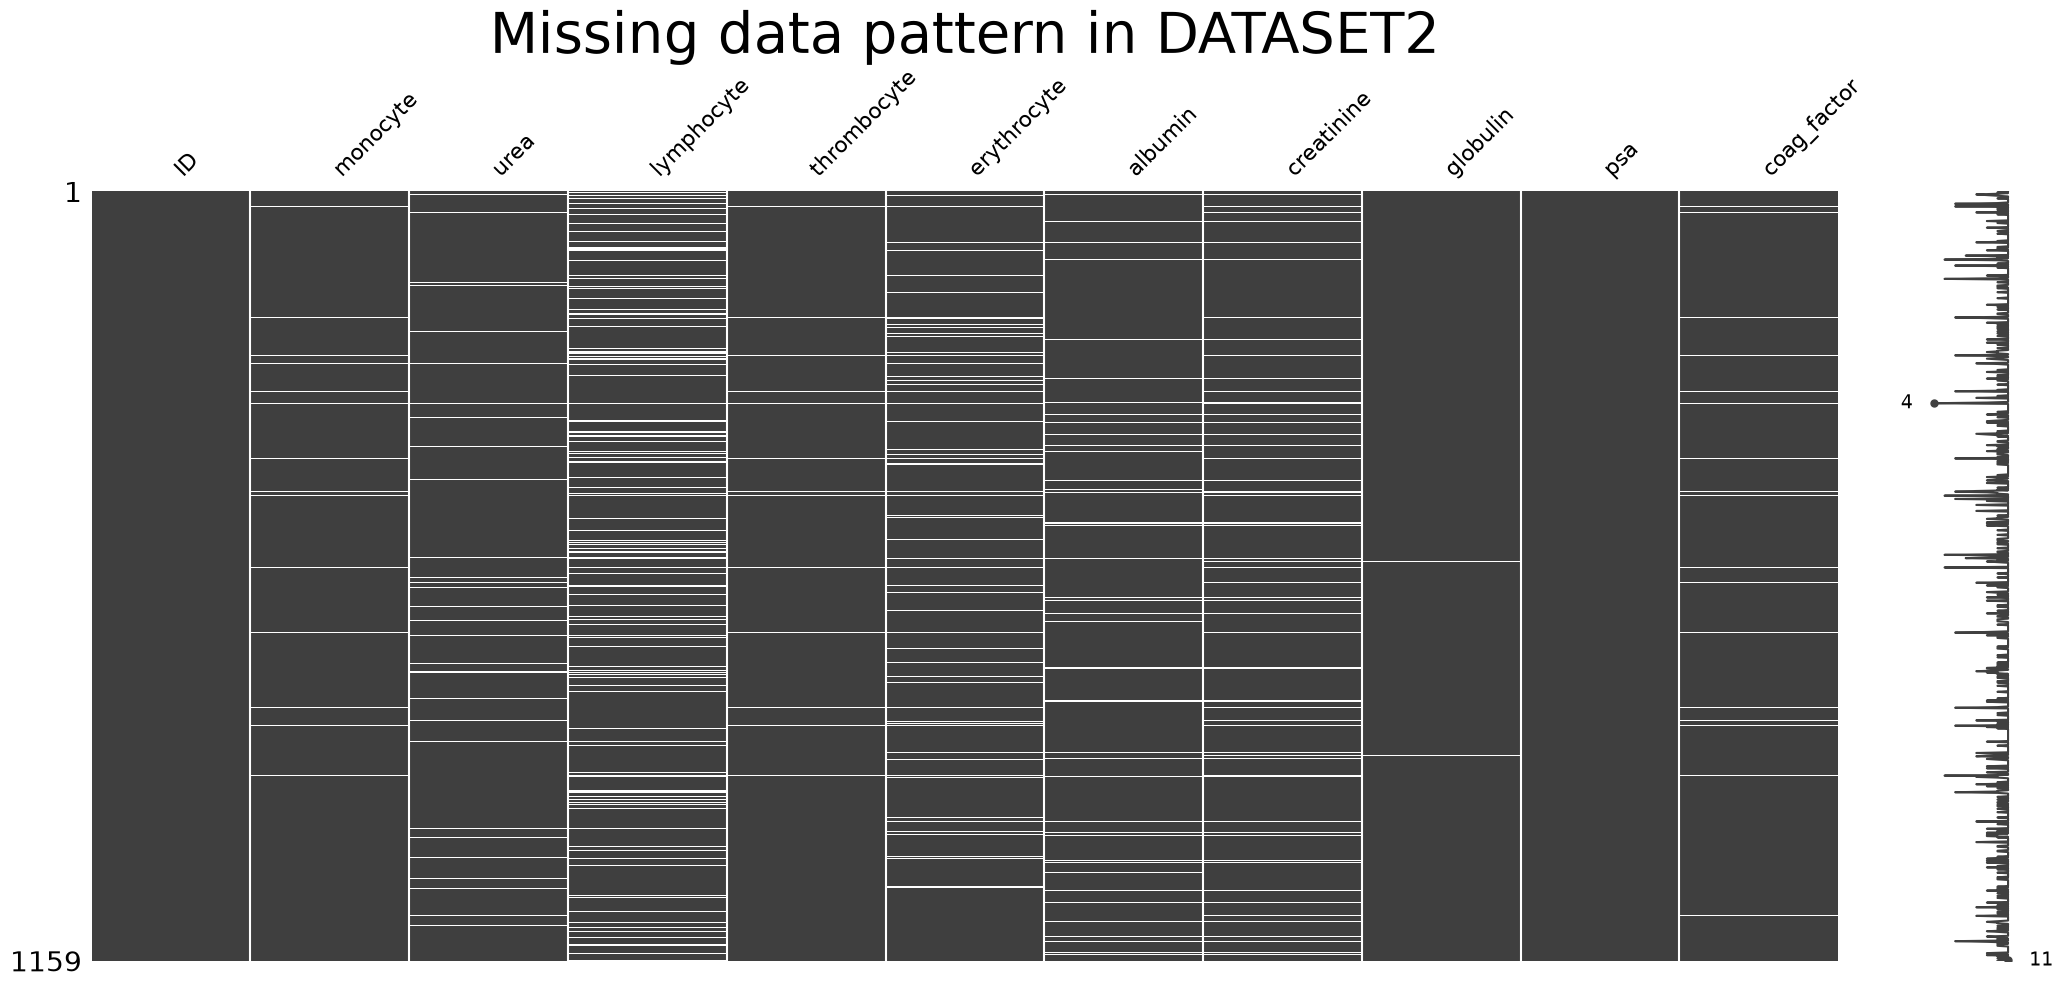
\includegraphics[width=\linewidth]{Images/missing_matrix.png}
\caption{Missingness pattern across DATASET2. Gaps are scattered rather than block-structured, consistent with values missing at random rather than missing systematically for a patient subgroup.}
\label{fig:missmat}
\end{figure}
\end{document}